\documentclass[10pt]{article}

% Specify the margins and text size.
\setlength{\textwidth}{6.4in}
\setlength{\textheight}{9.5in}
\setlength{\oddsidemargin}{0pt}
\setlength{\evensidemargin}{0pt}
\setlength{\topmargin}{0pt}
\setlength{\hoffset}{.05in}
\setlength{\voffset}{-1in}

\setlength{\parskip}{5pt}
\setlength{\parindent}{0pt}

% Load some fonts and symbol packages
\usepackage{latexsym}
\usepackage{pifont}       % contains 'star' symbol for counterinsurgency handbook title
\usepackage{yfonts} 
\usepackage{amsmath}
\usepackage{amsfonts}

\usepackage{graphicx}     % actually, this is loaded by pstricks
\usepackage[T1]{fontenc}
\usepackage{ifthen}
\usepackage{pstricks,pst-grad,pst-text,pst-node,multido,pst-plot,calc,pst-3dplot}
%\usepackage[all]{xy}
%\usepackage{animate}

% The hyperref package inserts links into the pdf.
\definecolor{MyLinkColor}{rgb}{.1,.2,1}
\definecolor{MyCiteColor}{rgb}{.1,1,.2}
\definecolor{MyURLColor}{rgb}{.4,.4,.4}
\usepackage[backref=true,pagebackref=false,hyperindex,colorlinks=true,
  linkcolor=MyLinkColor,urlcolor=MyURLColor]{hyperref}


% The tweaklist package is something I found on the web.  It provides a simple interface
% for making changes to spacing used in the itemize and enumerate environments.  Comment
% this out if you don't care to use tweaklist.
\usepackage{tweaklist}
\renewcommand{\itemhook}{\setlength{\parskip}{2pt}\setlength{\parsep}%
{1pt}\setlength{\topsep}{0pt}\setlength{\itemsep}{0pt}}

\newcommand{\U}{\underline{\hspace{5pt}}}

\usepackage{listings}
\newcommand{\Z}{\hphantom{0}}

\begin{document}
\pagestyle{empty}
\lstset{language=R, showspaces=false, showstringspaces=false}

\href{http://www.shepherd.edu}{
\includegraphics[height=1.75cm]{logo-high-res.eps}}
\vspace{-1.69cm}

{\small
\begin{tabular}{cl}
& Math 314\\
& Statistics\\
\hspace{5.28in} & %30 September 2011
\end{tabular}
}
\setlength{\baselineskip}{1.05\baselineskip}

\begin{center}
\textbf{\large  Regression Review Exercises}
\end{center}
\medskip

1. The length of odontoblasts (tooth cells) in each of 10 guinea pigs 
at each of three dose levels of vitamin~C (0.5, 1, and 2 mg) 
is measured.  The scatter plot of the data is shown below.

\begin{center}
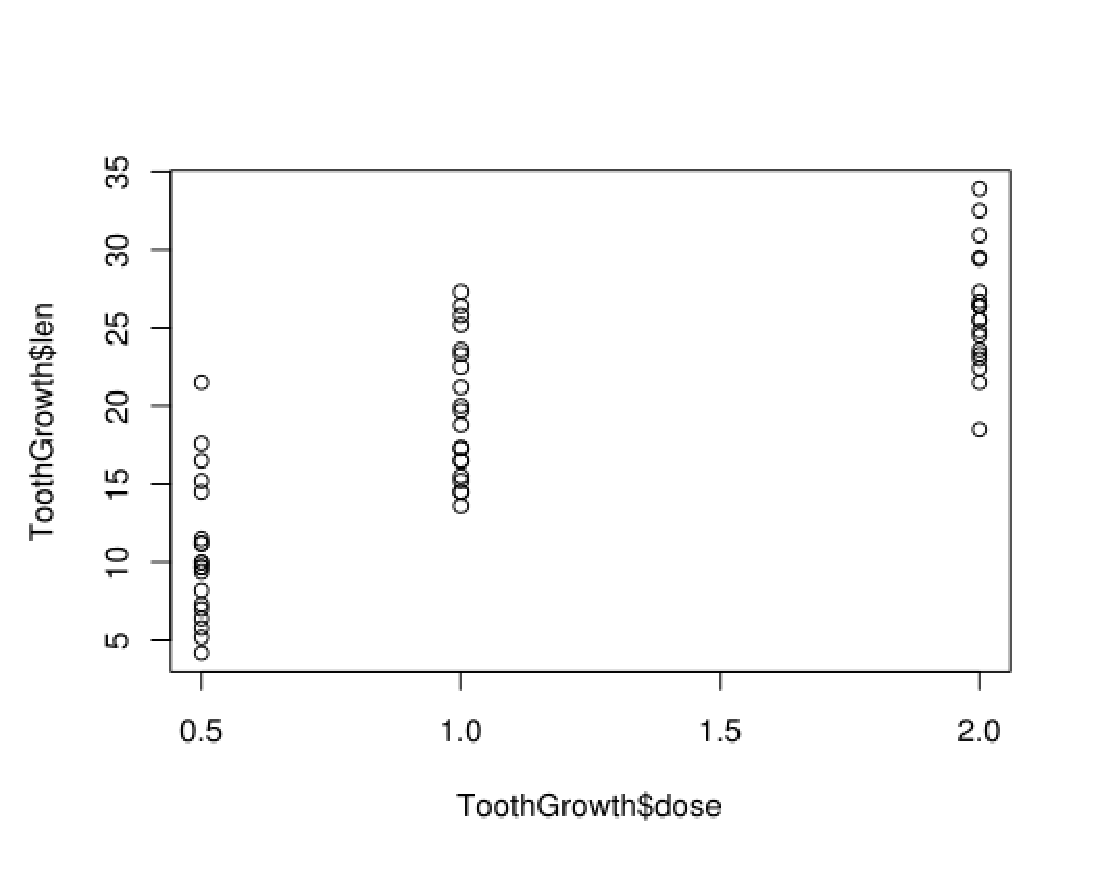
\includegraphics[height=1.75in,bb=0 22 515 340, clip]{teeth.eps}
\end{center}
The equation for the regression line computed from the data is 
\[y \approx 10\,x + 7\]
where $x$ is dose level in mg and $y$ is odontoblast length.
The correlation coefficient for the data is $r\approx 0.8$.

\hspace{20pt} a) Sketch the regression line in the above plot.
\medskip

\hspace{20pt} b) Estimate the odontoblast length if the dose level is $1.5$ mg.
\vspace{1.4in}

\hspace{20pt} c) The RMS error for the regression line is $4.5$.
Among guinea pigs that receive a vitamin C dose level of 1 mg, 68\% 
  have odontoblast length in what range?
\vspace{1.2in}

\hspace{20pt} d) One measurement has $\mbox{dose}=2.0$ mg and 
$\mbox{length}=23.0$. Calculate the length predicted by the regression
line then calculate the error (residual) for that value.
\vfill
\eject

2. For men age 25--34, the relationship between education (years of schooling
completed) and systolic blood pressure can be summarized as follows.
\begin{align*}
\mbox{average education} &\approx 13 \mbox{ years},
  & \mbox{SD} &\approx 3 \mbox{ years}\\
\mbox{average blood pressure} &\approx 119 \mbox{ mm}
  & \mbox{SD} &\approx 12 \mbox{ mm}
\end{align*}
The correlation coefficient is $r\approx -0.1$.

\hspace{20pt} a) Sketch the regression curve and the SD curve.
Write down the equations for both curves.
\vspace{2.5in}

\hspace{20pt} b) Predict the blood pressure of a man with 20 years of education.
\vspace{1.5in}

\hspace{20pt} c) One subject  had 20 years of education, and his 
blood pressure was 118~mm.  True or false and explain:  compared to other men
at his educational level, his blood pressure was a bit on the high side.
\vspace{1.4in}

\hspace{20pt} d) Suggest reasons for the sign and magnitude of $r$.
\vfill
\eject          

\end{document}

